\documentclass[11pt]{article}
\usepackage{amssymb}
\usepackage{amsthm}
\usepackage{enumitem}
\usepackage{physics,amsmath}
\usepackage{bm}
\usepackage{adjustbox}
\usepackage{mathrsfs}
\usepackage{graphicx}
\usepackage{siunitx}
\usepackage[mathscr]{euscript}


\title{\textbf{Solved selected problems of General Relativity - Thomas A. Moore}}
\author{Franco Zacco}
\date{}

\addtolength{\topmargin}{-3cm}
\addtolength{\textheight}{3cm}

\newcommand{\hatr}{\bm{\hat{r}}}
\newcommand{\hatn}{\bm{\hat{n}}}
\newcommand{\hatx}{\bm{\hat{x}}}
\newcommand{\haty}{\bm{\hat{y}}}
\newcommand{\hatz}{\bm{\hat{z}}}
\newcommand{\hatth}{\bm{\hat{\theta}}}
\newcommand{\hatphi}{\bm{\hat{\phi}}}
\newcommand{\hatrho}{\bm{\hat{\rho}}}
\newcommand{\er}{\bm{e}_r}
\newcommand{\etht}{\bm{e}_\theta}
\newcommand{\sci}[1]{\times 10^{#1}}

\theoremstyle{definition}
\newtheorem*{solution*}{Solution}
\renewcommand*{\proofname}{Solution}

\begin{document}
\maketitle
\thispagestyle{empty}

\section*{Chapter 15 - Alternative Coordinates}

\begin{proof}{\textbf{BOX 15.1} - Exercise 15.1.1.}\\
We know that 
\begin{align*}
    dt_d = \frac{dr}{(1-2GM/r)\sqrt{2GM/r}} \qquad
    d\tau = -\sqrt{\frac{r}{2GM}}dr
\end{align*}
Then $\partial\mathring{t}/\partial r = (dt_d + d\tau)/dr$ is
\begin{align*}
    \pdv{\mathring{t}}{r}
    &= \frac{1}{dr}\bigg(
        \frac{dr}{(1-2GM/r)\sqrt{2GM/r}} - \sqrt{\frac{r}{2GM}}dr
    \bigg)\\
    &= \frac{1 - (1-2GM/r)}{(1-2GM/r)\sqrt{2GM/r}}\\
    &= \frac{2GM/r}{(1-2GM/r)\sqrt{2GM/r}}\\
    &= \frac{\sqrt{2GM/r}}{(1-2GM/r)}
\end{align*}
\end{proof}

\cleardoublepage
\begin{proof}{\textbf{BOX 15.2} - Exercise 15.2.1.}\\
Let
\begin{align*}
    dt &= d\mathring{t} - \sqrt{\frac{2GM}{r}}\bigg(1 - \frac{2GM}{r}\bigg)^{-1}dr
\end{align*}
Then substituting $dt$ in
\begin{align*}
    ds^2 &= -\bigg(1 - \frac{2GM}{r}\bigg)dt^2 + \frac{dr^2}{1 - 2GM/r}
    + r^2(d\theta^2 + \sin^2\theta d\phi^2)
\end{align*}
We get that
\begin{align*}
    ds^2
    &= -\bigg(1 - \frac{2GM}{r}\bigg)\bigg(
        d\mathring{t} - \sqrt{\frac{2GM}{r}}\bigg(1 - \frac{2GM}{r}\bigg)^{-1}dr
    \bigg)^2
    + \bigg(1 - \frac{2GM}{r}\bigg)^{-1}dr^2\\
    &\quad+ r^2(d\theta^2 + \sin^2\theta d\phi^2)\\
    &= -\bigg(1 - \frac{2GM}{r}\bigg)d\mathring{t}^2
    + 2\sqrt{\frac{2GM}{r}}d\mathring{t}dr
    - \frac{2GM}{r}\bigg(1 - \frac{2GM}{r}\bigg)^{-1}dr^2
    + \bigg(1 - \frac{2GM}{r}\bigg)^{-1}dr^2\\
    &\quad+ r^2(d\theta^2 + \sin^2\theta d\phi^2)\\
    &= -\bigg(1 - \frac{2GM}{r}\bigg)d\mathring{t}^2
    + 2\sqrt{\frac{2GM}{r}}d\mathring{t}dr
    + \bigg(1 - \frac{2GM}{r}\bigg)^{-1}dr^2\bigg(1 - \frac{2GM}{r}\bigg)\\
    &\quad+ r^2(d\theta^2 + \sin^2\theta d\phi^2)\\
    &= -\bigg(1 - \frac{2GM}{r}\bigg)d\mathring{t}^2
    + 2\sqrt{\frac{2GM}{r}}d\mathring{t}dr + dr^2
    + r^2(d\theta^2 + \sin^2\theta d\phi^2)
\end{align*}
\end{proof}

\cleardoublepage
\begin{proof}{\textbf{BOX 15.3} - Exercise 15.3.1.}\\
We want to solve the following quadratic formula
\begin{align*}
    \bigg(\frac{2GM}{r} - 1\bigg) + 2\sqrt{\frac{2GM}{r}}\dv{r}{\mathring{t}}
    + \left(\dv{r}{\mathring{t}}\right)^2 = 0
\end{align*}
Then 
\begin{align*}
    \dv{r}{\mathring{t}}
    &= \frac{-2\sqrt{\frac{2GM}{r}} 
    \pm \sqrt{4\frac{2GM}{r} - 4\big(\frac{2GM}{r} - 1\big)}}{2}\\
    &= -\sqrt{\frac{2GM}{r}}
    \pm \sqrt{\frac{2GM}{r} - \bigg(\frac{2GM}{r} - 1\bigg)}\\
    &= -\sqrt{\frac{2GM}{r}} \pm 1
\end{align*}
\end{proof}
\begin{proof}{\textbf{BOX 15.4} - Exercise 15.4.1.}\\
Let
\begin{align*}
    u^2 - v^2 = \bigg(\frac{r}{2GM} - 1\bigg)e^{r/2GM}
\end{align*}
Then taking differentials on both sides we have that
\begin{align*}
    d(u^2 - v^2) &= d\bigg(\bigg(\frac{r}{2GM} - 1\bigg)e^{r/2GM}\bigg)\\
    2udu - 2vdv
    &= \frac{e^{r/2GM}(2GM + r)}{(2GM)^2}dr - \frac{e^{r/2GM}}{2GM}dr\\
    2(udu - vdv)
    &= \frac{re^{r/2GM}}{(2GM)^2}dr
\end{align*}
Hence
\begin{align*}
    \frac{re^{r/2GM}}{(2GM)^2}dr &= 2(udu - vdv)\\
    dr &= \frac{8(GM)^2}{r}e^{-r/2GM}(udu - vdv)
\end{align*}
\end{proof}

\cleardoublepage
\begin{proof}{\textbf{BOX 15.4} - Exercise 15.4.2.}\\
For the case $u + v > 0$, $u - v > 0$ we have that
\begin{align*}
    t = 2GM\ln(u + v) - 2GM\ln(u - v)
\end{align*}
Then taking differentials on both sides gives us
\begin{align*}
    dt &= d(2GM\ln(u + v) - 2GM\ln(u - v))\\
    dt &= \frac{2GM}{u + v}du + \frac{2GM}{u + v}dv - \frac{2GM}{u - v}du
    + \frac{2GM}{u - v}dv\\
    dt &= \frac{2GM}{u + v}(du + dv) - \frac{2GM}{u - v}(du - dv)\\
    dt &= 2GM\bigg(\frac{du + dv}{u + v} - \frac{du - dv}{u - v}\bigg)
\end{align*}
\end{proof}

\cleardoublepage
\begin{proof}{\textbf{BOX 15.4} - Exercise 15.4.3.}\\
Squaring equation 15.18 gives us
\begin{align*}
    dr^2 &= \frac{64(GM)^4}{r^2}e^{-r/GM}(udu - vdv)^2
\end{align*}
And squaring equation 15.21 gives us
\begin{align*}
    dt^2 &= \frac{16(GM)^2e^{-r/GM}}{(r/2GM - 1)^2}(udv - vdu)^2
\end{align*}
Then we have that
\begin{align*}
    &-\bigg(1 - \frac{2GM}{r}\bigg)dt^2 + \bigg(1 - \frac{2GM}{r}\bigg)^{-1}dr^2 = \\
    %
    &\quad = -\bigg(1 - \frac{2GM}{r}\bigg)
    \frac{16(GM)^2e^{-r/GM}}{(r/2GM - 1)^2}(udv - vdu)^2\\
    &\qquad + \bigg(1 - \frac{2GM}{r}\bigg)^{-1}
    \frac{64(GM)^4}{r^2}e^{-r/GM}(udu - vdv)^2\\
    %
    &\quad = -\frac{r - 2GM}{r}
    \frac{16(GM)^2e^{-r/GM}}{(r - 2GM)^2/(2GM)^2}(udv - vdu)^2\\
    &\qquad + \frac{r}{r - 2GM}
    \frac{64(GM)^4}{r^2}e^{-r/GM}(udu - vdv)^2\\
    %
    &\quad = -\frac{64(GM)^4e^{-r/GM}}{r(r - 2GM)}(udv - vdu)^2
    + \frac{64(GM)^4e^{-r/GM}}{r(r - 2GM)}(udu - vdv)^2\\
    %
    &\quad = \frac{64(GM)^4e^{-r/GM}}{r(r - 2GM)}
    (-u^2dv^2 + 2uvdudv - v^2du^2 + u^2du^2 - 2uvdudv + v^2dv^2)\\
    %
    &\quad = \frac{64(GM)^4e^{-r/GM}}{r(r - 2GM)}(u^2 - v^2)(du^2 - dv^2)\\
    %
    &\quad = \frac{64(GM)^4e^{-r/GM}}{r(r - 2GM)}\frac{r - 2GM}{2GM}e^{r/2GM}(du^2 - dv^2)\\
    %
    &\quad = \frac{32(GM)^3e^{-r/2GM}}{r}(du^2 - dv^2)
\end{align*}

\end{proof}

\cleardoublepage
\begin{proof}{\textbf{P15.1}}
\begin{itemize}
\item [\textbf{a.}] Given an observer (a robot) falling from rest has $e = 1$
we get that
\begin{align*}
    \bigg(1 - \frac{2GM}{r}\bigg)\dv{t}{\tau} &= 1\\
    \dv{t}{\tau} &= \bigg(1 - \frac{2GM}{r}\bigg)^{-1}
\end{align*}
Also, $l = 0$ since it's falling radially, so $d\phi/d\tau = 0$ so the
equation of motion becomes
\begin{align*}
    \frac{1}{2}\bigg(\dv{r}{\tau}\bigg)^{2} - \frac{GM}{r} &= 0\\
    \dv{r}{\tau} &= \pm\sqrt{\frac{2GM}{r}}
\end{align*}
Finally, if we assume this to happen on the equatorial plane must be that
$d\theta/d\tau = 0$. Therefore, the robot observer's time basis vector
expressed in Schwarzschild coordinates is
\begin{align*}
    (\bm{o}_{\mathring{t}})^\mu &= \begin{bmatrix}
        \big(1 - \frac{2GM}{r}\big)^{-1}\\[7pt]
        -\sqrt{\frac{2GM}{r}}\\[7pt]
        0\\[7pt] 0
    \end{bmatrix}
\end{align*}
\item [\textbf{b.}] Now, let us compute
$d\mathring{t} = -\bm{o}_{\mathring{t}}\cdot d\bm{s}$ as follows
\begin{align*}
    d\mathring{t} &= -\bm{o}_{\mathring{t}}\cdot d\bm{s}\\
    &= -(g_{tt}(\bm{o}_{\mathring{t}})^t d\bm{s}^t + g_{rr}(\bm{o}_{\mathring{t}})^r d\bm{s}^r)\\
    &= -\bigg(
    -\bigg(1 - \frac{2GM}{r}\bigg)\bigg(1 - \frac{2GM}{r}\bigg)^{-1}dt
    - \bigg(1 - \frac{2GM}{r}\bigg)^{-1}\sqrt{\frac{2GM}{r}}dr
    \bigg)\\
    &= dt + \bigg(1 - \frac{2GM}{r}\bigg)^{-1}\sqrt{\frac{2GM}{r}}dr
\end{align*}
This is exactly the equation (15.4) as we wanted.
\end{itemize}
\end{proof}

\cleardoublepage
\begin{proof}{\textbf{P15.3}}
From BOX 15.3 we know that for a radial photon the rain-coordinate velocities
are
\begin{align*}
    \dv{r}{\mathring{t}} &= -\sqrt{\frac{2GM}{r}} \pm 1
\end{align*}
Hence, assuming the photon is ingoing (negative sign) and letting
$u = \sqrt{2GM/r}$ and $dr = -4GM/u^3~du$ we get that
\begin{align*}
    \int d\mathring{t} &= -\int \frac{dr}{u + 1}\\
    \int d\mathring{t} &= \int \frac{4GM}{u^3(u + 1)}~du\\
    \mathring{t}
    &= 4GM\bigg[-\frac{1}{2u^2} + \frac{1}{u} + \ln(\frac{u}{u + 1})\bigg] + C\\
    \mathring{t}
    &= 4GM\bigg[-\frac{1}{2u^2} + \frac{1}{u} - \ln(1 + \frac{1}{u})\bigg] + C\\
    \mathring{t}
    &= 4GM\bigg[
        -\frac{r}{4GM} + \sqrt{\frac{r}{2GM}} - \ln(1 + \sqrt{\frac{r}{2GM}})
    \bigg] + C\\
    \mathring{t} &= -r + \sqrt{8GMr} - 4GM\ln(1 + \sqrt{\frac{r}{2GM}}) + C
\end{align*}
In the following plot, we compare the worldlines of a free-falling robot and a
radial ingoing photon.
\begin{center}
    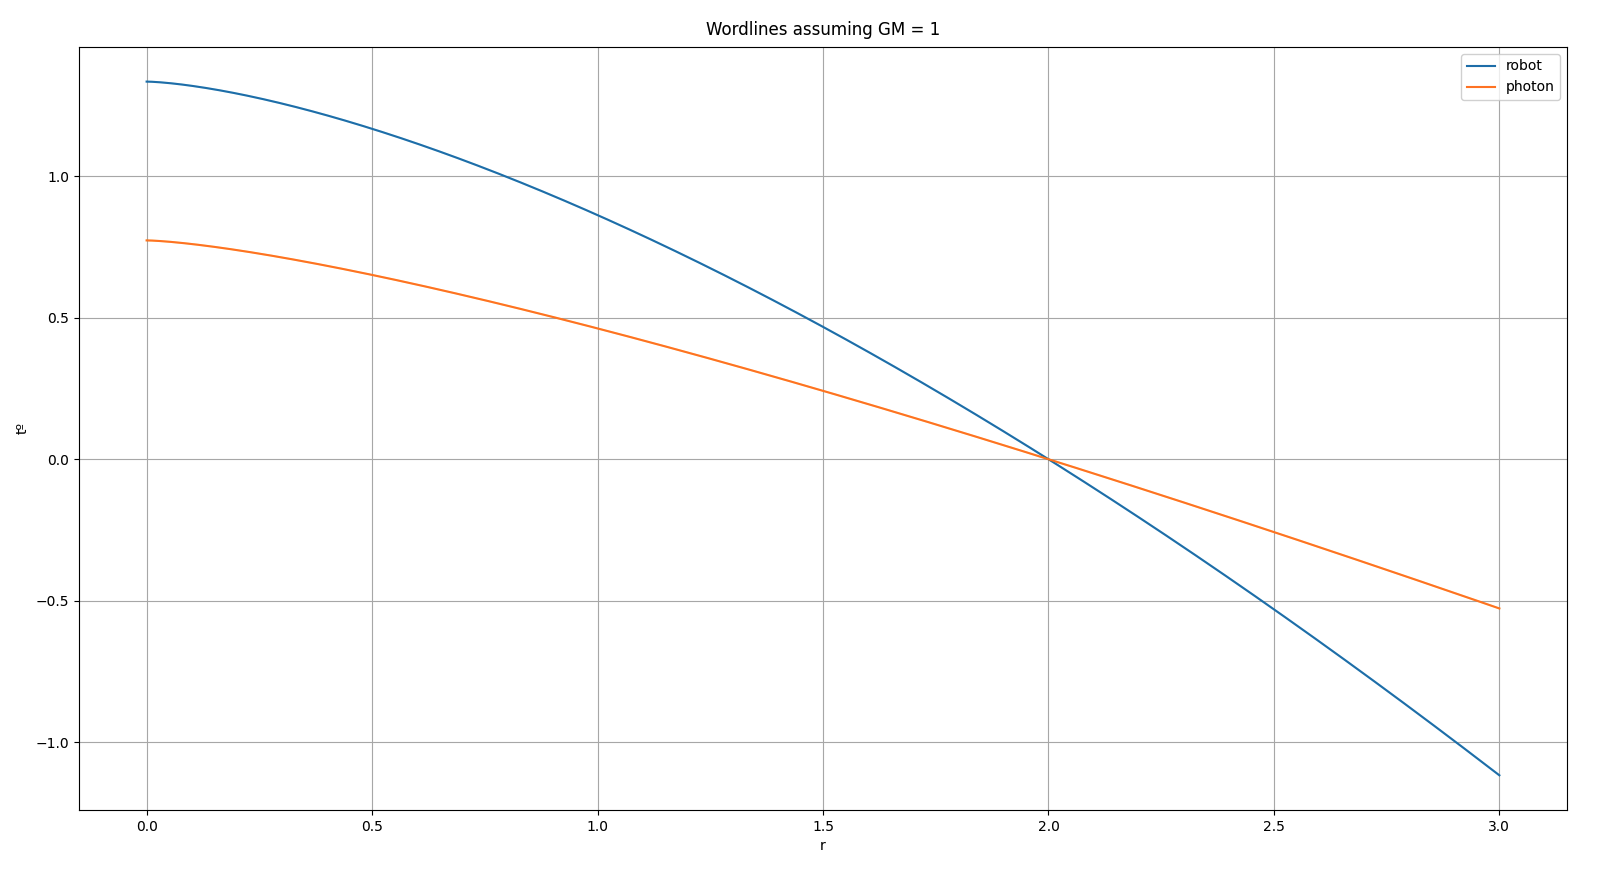
\includegraphics[scale=0.25]{ch15-p15.3.png}
\end{center}
\end{proof}

\cleardoublepage
\begin{proof}{\textbf{P15.4}}
The falling observer cannot see the future of the outside universe to infinity
because the lightcone when passing $r = 2GM$ is facing upward, so he cannot see
the outside future, but only "his" future.

Also, the observer is not completely cut off from the outside universe because
of the downward face of the lightcone, so some light can still be arriving from
the outside universe.
\end{proof}
\begin{proof}{\textbf{P15.5}}
Let us consider Figure 5.3.
\\
An outgoing photon follows a straight line path with slope +1 in the
Kruskal-Szekeres spacetime diagram, i.e. the right side of the lightcone.
\\
We see that a photon might meet us again only at $r = 0$ but not before since
the worldline we follow never crosses again the worldline the photon is following.
\end{proof}
\begin{proof}{\textbf{P15.6}}
Let us consider Figure 5.3.
\\
An outgoing photon follows a straight line worldline with slope +1 in the
Kruskal-Szekeres spacetime diagram, so even though photon worldlines might
cross the observer's worldline, the photons start at $r=0$ but $r$ cannot
grow (even for outgoing photons), so photons starting at $r=0$ will stay there.
\\
Therefore, observers falling through the event horizon won't see light from
the surface.
\end{proof}
\begin{proof}{\textbf{P15.7}}
No, we cannot go and rescue the wrench at any later time because the wrench
is a massive object, so it follows a worldline towards $r=0$ and eventually
will reach it.
\\
So we have a limited time (according to our watch) to catch it after it falls.
\end{proof}
\begin{proof}{\textbf{P15.8}}
Yes, there is a moment when the observers at the front of the ship cannot see
or receive signals from the tail end. This time is when the tail end has passed
the event horizon, but the front end has not passed yet.
\\
This is because no outgoing photon can escape the event horizon; they can only
travel towards $r=0$. 
\\
On the other hand, any signal or light emitted from the tail end at $r = 0$
will stay there since it cannot travel towards a greater $r$, this implies 
that the front end cannot see or receive any signal from the tail end when
the tail end has reached $r = 0$.
\end{proof}

\cleardoublepage
\begin{proof}{\textbf{P15.9}}
\begin{itemize}
\item [\textbf{a.}] Given that
\begin{align*}
    \bigg(\frac{R}{2GM} - 1\bigg)e^{R/2GM} = 1
\end{align*}
Then this means that $u^2 - v^2 = 1$ for the spaceship so the hyperbola of
constant $r$ must cross the u-axis at $1$ and hence the KS spacetime diagram
looks like the following
\begin{center}
    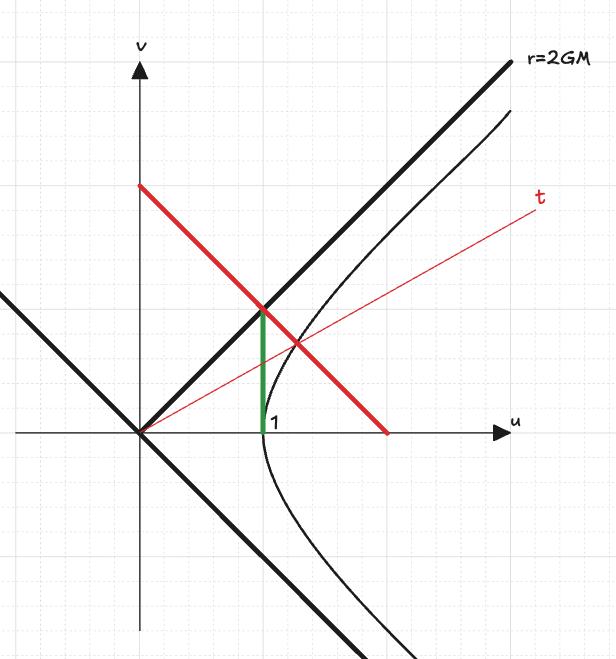
\includegraphics[scale=0.35]{ch15-p15.9.png}
\end{center}
Where the green line is the path of the spacecraft.

\item [\textbf{b.}] From the previous plot, we see that for reaching the
shuttle at the event horizon (the latest time) the ship must travel at the
speed of light following the bold red worldline.
From the plot we see that this line has the following equation
\begin{align*}
    v = -u + 2
\end{align*}
But also the ship departs from the same $R$ so it must also satisfy
$u^2 - v^2 = 1$ then
\begin{align*}
    u^2 - v^2 &= 1\\
    u^2 &= 1 + (2 - u)^2\\
    u^2 &= 5 - 4u + u^2\\
    u &= \frac{5}{4}
\end{align*}
Now we determine $t$ as follows
\begin{align*}
    t = 2GM \ln(\frac{u + (2 - u)}{2u -2}) = 2GM \ln(\frac{2}{\frac{5}{2} - 2})
    = 2.772 GM
\end{align*}
\end{itemize}
\end{proof}

\end{document}